\documentclass{standalone}
\usepackage{tikz}
\usepackage{mathrsfs}
\usetikzlibrary{positioning, shapes.geometric, arrows}
\usepackage[T1]{fontenc}
\renewcommand*\familydefault{\ttdefault} %% Only if the base font of the document is to be typewriter style
\begin{document}
	 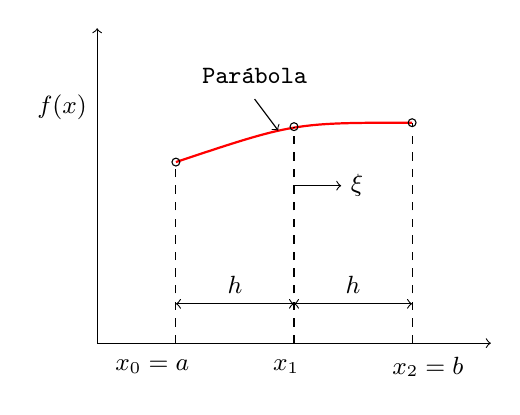
\begin{tikzpicture}[font=\small]
		\draw [->] (0,0) -- node [near end, left] {$f(x)$}(0,4);
		\draw [->] (0,0) -- (5,0);
		\draw [red, thick] (1,2.3) .. controls (2.5,2.8) ..  (4,2.8);
		%\draw (1,2.3) -- (4,2.8);
		\draw [dashed] (1,0) -- (1,2.3);
		\draw [dashed] (2.5,0) -- (2.5,2.75);
		\draw [dashed] (4,0) -- (4,2.8);
		\draw (1,2.3) circle (0.05);
		\draw (2.5,2.75) circle (0.05);
		\draw (4,2.8) circle (0.05);
		\draw [<->] (1,0.5) -- node [midway, above] {$h$} (2.5,0.5);
		\draw [<->] (2.5,0.5) -- node [midway, above] {$h$} (4,0.5);
		\draw (3.3,2) node {$\xi$};
		\draw [->](2.5,2) -- (3.1,2);
		\draw (0.7,-0.3) node {$x_{0}=a$};
		\draw (2.4,-0.3) node {$x_{1}$};
		\draw (4.2,-0.3) node {$x_{2}=b$};
		%\draw (2.2,1.7) node {Area=I};
		\draw (2,3.4) node {Parábola};
		\draw [->] (2,3.1) -- (2.3,2.7);
\end{tikzpicture}
\end{document}